\chapter{Sistemi dinamici TC}
Un sistema dinamico è descritto formalmente dalla seguente \emph{8-upla}: 
\begin{equation}
	(T,\mathcal{U},U,\mathcal{Y},Y,X,\phi, \psi)
\end{equation}

con:
\begin{itemize}
	\item T $\subset \mathbb{R}$ è l'insieme dei tempi (che in questo caso è $\mathbb{R}$ perchè è a TC).
	\item $\mathcal{U}$ è l'insieme dei segnali di ingresso, $u(t):T\longrightarrow U$ con $U$ l'insieme dei possibili valori di ingresso.
	\item $\mathcal{Y}$ è l'insieme dei segnali di uscita, $y(t): T \longrightarrow Y$ con $Y$ l'insieme dei valori di uscita.
	\item $X$ è l'insieme dei valori possibili per lo stato del sistema.
	\item $\phi$ è la mappa di transizione globale dello stato:
	\begin{equation}
		\phi(t,\tau,x(t),u_{[t,\tau]}) \longrightarrow x(\tau)
	\end{equation}
	\item $\psi$ è la mappa di transizione globale dell'uscita:
	\begin{equation}
		\psi(t,\tau,x(t),u_{[t,\tau]}) \longrightarrow y(\tau)
	\end{equation}
\end{itemize}

\paragraph{}
Definiamo lo \emph{stato del sistema} come il vettore di n componenti che caratterizza completamente la situazione attuale del sistema dinamico:
\begin{equation}
	\underline{x}(t): T \longrightarrow X
\end{equation}
\paragraph{}
Una tipica rappresentazione di questi sistemi dinamici è la \emph{I/S/U locale} che consiste nel mappare lo stato attraverso la funzione $f$ e mappare l'uscita attraverso la funzione $g$. Quindi questa rappresentazione si ottiene sostituendo nella ($B.1$) $\phi$ con $f$ e $\psi$ con $g$.\\ 
Pertanto l'evoluzione del sistema dinamico a TC si ottiene dalle seguenti equazioni:
\begin{equation}
	\begin{cases}
		\underline{\dot{x}} = \underline{f}(t, \underline{x}(t), \underline{u}(t)) \\
		\underline{y} = \underline{g}(t, \underline{x}(t), \underline{u}(t)) \\
	\end{cases}
\end{equation}
con $\underline{x}(t)$ stati, $\underline{y}(t)$ uscite e $\underline{u}(t)$ ingressi
\begin{center}
	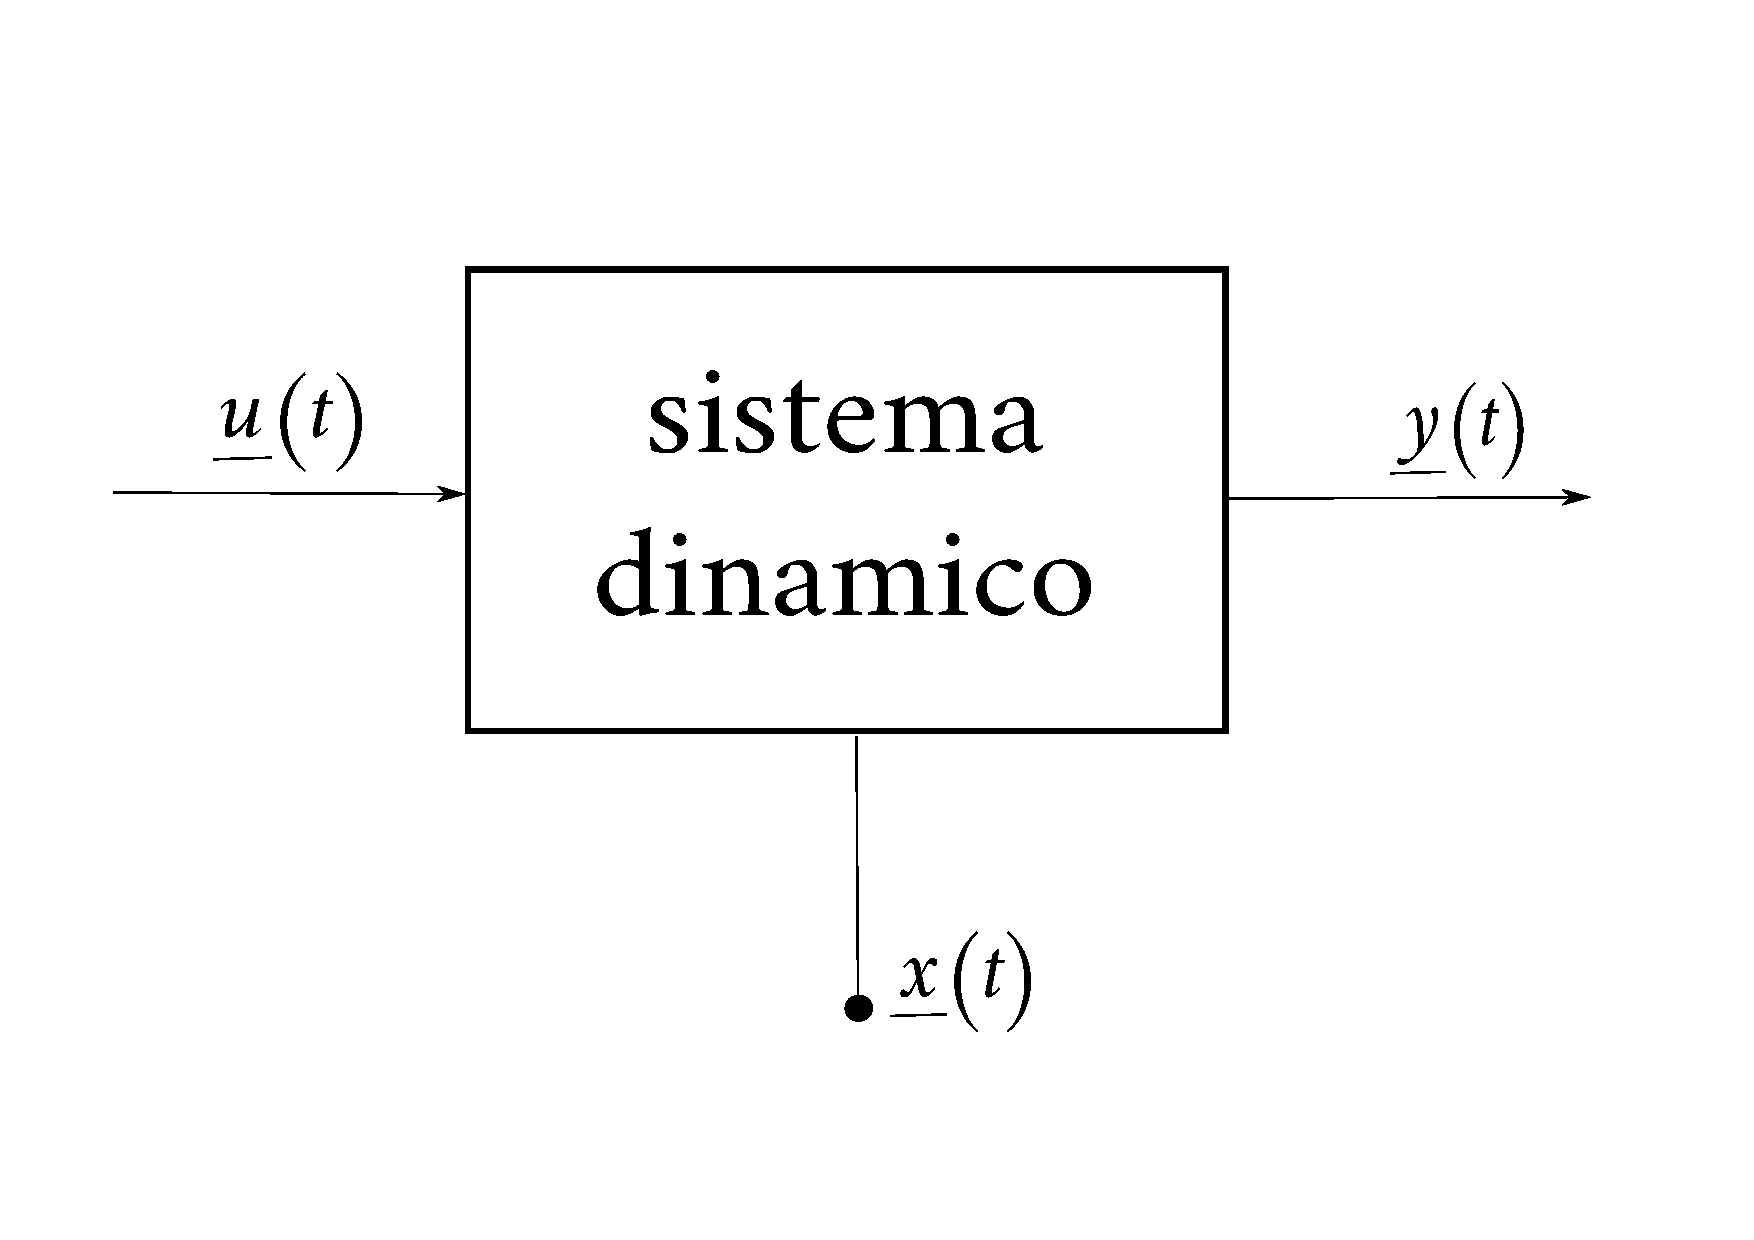
\includegraphics[scale=0.2]{sistemaDinamico.pdf}
	\captionof{figure}{sistema dinamico}
\end{center}
e notiamo che:
\begin{itemize}
	\item Se non c'è la dipendenza da $t$, il sistema si dice \emph{tempo-invariante}.
	\item Se non c'è la dipendenza da $\underline{u}(t)$ il sistema si dice \emph{autonomo}.
	\item Un sistema si dice \emph{lineare} se vale il principio di \emph{sovrapposizione degli effetti}.
\end{itemize}
In generale, studieremo un vettore $\underline{e}$ che chiameremo \emph{vettore errore} e l'obiettivo sarà quasi sempre quello di renderlo nullo, o meglio, anche se non dovesse essere nullo, vogliamo che $ \lim_{t \to \infty} \underline{e}(t) = \underline{0}$.

\section{Definizioni}
Passiamo in rassegna un po di definizioni per i sistemi dinamici:
\begin{itemize}
	\item Per il sistema autonomo $\underline{\dot{x}} = \underline{f}(\underline{x})$, si dice che $\underline{x}^{eq}$ è di \emph{equilibrio} se
	\begin{equation}
		\underline{f}(\underline{x}^{eq}) = \underline{0}
	\end{equation}	 
	\item Si definisce \emph{stabilità semplice o marginale} del sistema $\underline{\dot{x}} = \underline{f}(\underline{x})$ in cui assumiamo che l'origine sia un punto di equilibrio, ovvero che $\underline{f}(\underline{0}) = \underline{0}$ se
	\begin{equation}
		\forall B_{\varepsilon}, \varepsilon > 0,\: \exists B_{\delta}, \delta = \delta(\varepsilon) : \underline{x}(0)\in B_{\delta} \quad \Rightarrow \quad \underline{x}(t)\in B_{\delta} \;\; \forall t>0
	\end{equation}
	\item Si parla di \emph{convergenza} quando esiste un intorno aperto $I$ che contiene l'origine (punto di equilibrio) tale che:
	\begin{equation}
		\underline{x}(0)\in I \quad \Rightarrow \quad \lim_{t \to \infty} \underline{x}(t) = 0
	\end{equation}
	allora il sistema si dice convergente con \emph{dominio di attrazione} $I$.
	\item La \emph{stabilità asintotica} è l'unione della \emph{stabilità semplice} e \emph{convergenza}, infatti, il sistema è \emph{asintoticamente stabile} nell'origine se il suo \emph{dominio di attrazione} coincide con lo \emph{spazio di stato}.
\end{itemize}

\section{Sistemi LTI}
Supponiamo $dim(X) = n$, $dim(U) = m$, $dim(Y) = p$, i sistemi \emph{lineari e tempo-invarianti} (LTI), hanno come rappresentazione \emph{locale I/S/U} la seguente relazione matriciale:
\begin{equation}
	\begin{cases}
		\underline{\dot{x}}(t) = A\underline{x}(t) + B\underline{u}(t)
		\underline{y}(t) = C\underline{x}(t) + D\underline{u}(t)
	\end{cases}
\end{equation} 
con $A \in \mathbb{R}^{n \times n}$, $B \in \mathbb{R}^{n \times m}$, $C \in \mathbb{R}^{p \times n}$, $D\in\mathbb{R}^{p \times m}$.
\paragraph{}
Anche in questo caso enunciamo qualche concetto fondamentale,
\begin{itemize}
	\item Nei sistemi LTI autonomi $\underline{\dot{x}} = A\underline{x}$, quando cerchiamo i punti di equilibrio e sappiamo $\vert A \vert \neq 0$, l'unica soluzione al sistema lineare $A\underline{x} = \underline{0}$ è quella banale, ovvero $\underline{x} = \underline{0}$ e quindi esiste \emph{un solo} punto di equilibrio, cioè l'origine.
	\item Nei sistemi LTI autonomi si può ricavare dalla ($B.9$) la \emph{rappresentazione globale} dello stato:
\begin{equation}
	\begin{cases}
		\underline{x}(t) = e^{At}\underline{x}(0) \\
		\underline{y}(t) = Ce^{At}\underline{x}(0)\\
	\end{cases}
\end{equation}
notiamo che serve \emph{esponenziale di matrice} $e^{At}$, possiamo esprimerlo nel seguente modo,
\begin{equation}
	e^{At} = I + \frac{At}{1!} + \frac{A^2t^2}{2!} + \frac{A^3t^3}{3!} + \cdots
\end{equation}
e quindi derivando otteniamo,
\begin{equation}
	\frac{d}{dt}\Big( e^{At} \Big) = 0 + A + \frac{A^2t}{1!} + \frac{A^3t^2}{2!} + \cdots = A \Big( I + \frac{At}{1!} + \frac{A^2t^2}{2!} + \cdots \Big) = A e^{At}
\end{equation}
	\item La matrice $A$ è di fondamentale importanza per lo studio della stabilità, infatti, \emph{se tutti gli autovalori di A sono a parte reale negativa, il sistema è globalmente asintoticamente stabile.}
\end{itemize}

\section{Metodo diretto di Lyapunov}
La filosofia di questo metodo è analizzare le proprietà di stabilità senza risolvere le equazioni differenziali che descrivono il sistema dinamico. Sia il sistema autonomo $\underline{\dot{x}} = \underline{f}(\underline{x})$.\\ 
Se riusciamo a costruire una \emph{funzione scalare} dello stato $V(\underline{x}) > 0$ \emph{radialmente illimitata}, (ovvero: se $\vert\vert \underline{x} \vert\vert \longrightarrow \infty \; \Rightarrow \; V(\underline{x}) \longrightarrow \infty $). Enunciamo il seguente teorema:
\begin{itemize}
	\item Se $\dot{V}(\underline{x}) \leqslant 0$ \emph{allora} il sistema è \textbf{marginalmente stabile}.
	\item Se $\dot{V}(\underline{x}) < 0$ \emph{allora} il sistema è \textbf{asintoticamente stabile}.
\end{itemize}
\paragraph{}
Chiamiamo $V(\underline{x})$ la \emph{candidata di Lyapunov} e diventa effettivamente \emph{funzione di Lyapunov} se $V(\underline{x})$ è tale da rendere $\dot{V}(\underline{x}) \leqslant 0$. Quindi, il \emph{metodo di Lyapnov} consiste nel cercare un segnale di controllo $\underline{u}$ che renda $\leqslant 0$ la derivata di una cadidata di Lyapunov. Notiamo, che questo metodo esprime una condizione solo \emph{sufficiente} per la stabilità del sistema.

\section{Controllo in Retroazione}
Esaminiamo lo schema di controllo in retroazione in figura,
\begin{center}
	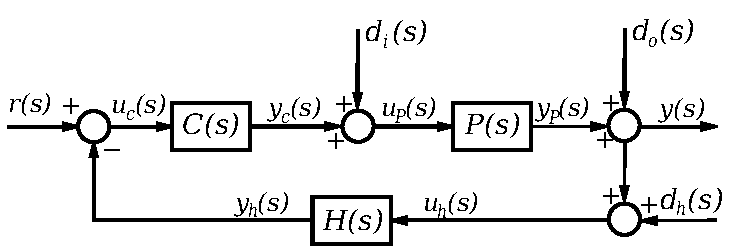
\includegraphics[scale=0.8]{ControlSystem.pdf}
	\caption{Schema di controllo generale.}
\end{center}
questo tipo di collegamento è utile perchè riesce a modificare la \emph{funzione di trasferimento} (f.d.t.) dell'impianto $P(s)$ governando i poli e zeri e poter soddisfare la \emph{reiezione dei disturbi} e \emph{inseguimento perfetto}. 

Lo schema precedente è equivalente al seguente schema a retroazione unitaria con la \emph{Loop transfer function} $L(s) = C(s)P(s)H(s)$,
\begin{center}
	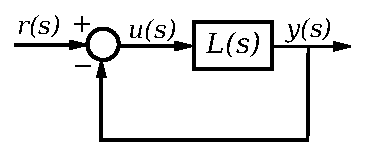
\includegraphics[scale=0.8]{ControlSystemLoop.pdf}
	\caption{Schema di controllo a retroazione unitaria.}
\end{center}

Inoltre possiamo ridurre ancora lo schema riducendo tutto il sistema ad un unico blocco $W(s) = \frac{L(s)}{1 + L(s)}$
\begin{center}
	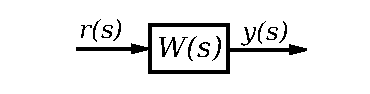
\includegraphics[scale=0.8]{ControlSystemW.pdf}
	\caption{Sistema equivalente monoblocco.}
\end{center}

\section{Luogo delle radici}
Il luogo delle radici è un metodo grafico, sviluppato da \emph{Evans} nel 1948, per l'analisi e il progetto di sistemi di controllo. Consente di visualizzare i luoghi percorsi dai \emph{poli} in anello chiuso del sistema di controllo al variare del \emph{guadagno d'anello}. 

Sia il sistema retroazionato in figura
\begin{center}
	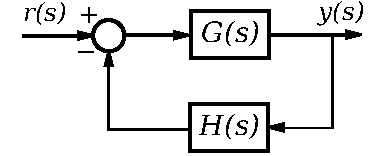
\includegraphics[scale=0.6]{ControlSystemRadici.pdf}
	\caption{Sistema retroazionato.}
\end{center}
con $n$ poli e $m$ zeri, scriviamo la funzione ad anello $L(s)$
\begin{equation}
	L(s) = G(s)H(s) = k \frac{b(s)}{a(s)} = k \frac{ \prod_{j=1}^{m} (s - z_j)}{ \prod_{i = 1}^{n} (s - p_i)}
\end{equation}
con $z_j$ zeri del sistema, $p_i$ poli del sistema e $n \geqslant m$ perchè il sistema è \emph{causale}.

Otteniamo la seguente \emph{f.d.t.} del sistema
\begin{equation}
	\frac{y(s)}{r(s)} = \frac{G(s) a(s)}{a(s) + k b(s)}
\end{equation}

\subsubsection{Le proprietà del luogo delle radici che ne permettono il \emph{tracciamento} sono:}

\begin{enumerate}
	\item Il luogo delle radici è simmetrico rispetto all'asse reale.
	\item Tutti i punti dell'asse reale appartengono al luogo delle radici, in particolare:
	\begin{enumerate}
		\item Al \emph{luogo positivo} appartengono tutti i punti dell'asse reale che lasciano alla propria destra un numero dispari di singolarità (poli e zeri) contate con la loro molteplicità.
		\item Al \emph{luogo negativo} appartengono tutti i punti dell'asse reale che lasciano alla propria destra un numero pari di singolarità (poli e zeri) contate con la loro molteplicità 
	\end{enumerate}
	\item Il luogo delle radici è costituito da $n$ rami ed eventuali intersezioni vanno determinate per un determinato valore di $k$ e corrispondono ai poli multipli della $L(s)$.
	\item Per $k \rightarrow 0$ otteniamo:
	\begin{enumerate}
		\item Gli $n$ rami del \emph{luogo positivo} partono dai poli.
		\item Gli $n$ rami del \emph{luogo negativo} finiscono ai poli.
	\end{enumerate}
	\item Per il comportamento asintotico abbiamo:
	\begin{enumerate}
		\item Per $k \rightarrow \infty$ gli $m$ rami del \emph{luogo positivo} finiscono agli zeri.
		\item Per $k \rightarrow -\infty$ gli $m$ rami del \emph{luogo negativo} partono dagli zeri.
		\item I rimanenti $n-m$ rami del \emph{luogo positivo} divergono verso $n-m$ asintoti all'infinito.
		\item I rimanenti $n-m$ rami del \emph{luogo negativo} provengono dall'infinito da $n-m$ asintoti.
	\end{enumerate}
	\item Gli asintoti formano una \emph{stella} di centro sull'asse reale in 
		\begin{equation}
			\sigma = \frac{\sum_{i = 1}^{n}p_i - \sum_{j = 1}^{m}z_j}{n-m}
		\end{equation}
	\item Le \emph{direzioni} degli asintoti sono dovute all'inclinazione rispetto l'asse reale che sono date da:
	\begin{enumerate}
		\item Per il \emph{luogo positivo} con $k>0$,
			\begin{equation}
				\vartheta = \frac{(2\alpha + 1) \pi}{n-m} \qquad \alpha = 0,1,\cdots,n-m-1
			\end{equation}
		\item Per il \emph{luogo negativo} con $k<0$,
			\begin{equation}
				\vartheta = \frac{2\alpha \pi}{n-m} \qquad \alpha = 0,1,\cdots,n-m-1
			\end{equation}
	\end{enumerate}
	\item I \emph{punti di diramazione} del luogo, ovvero i punti in cui il luogo abbandona l'asse reale si ottengono, sia per il luogo positivo che quello negativo, risolvendo la seguente equazione,
		\begin{equation}
			\frac{d}{ds} \Bigl[ 1 + G(s)H(s) \Bigr] = 0
		\end{equation}
\end{enumerate}

\subsubsection{Esempio}
Supponiamo di voler calcolare il luogo delle radici del sistema con la seguente $L(s)$
\begin{equation}
	L(s) = G(s)H(s) = \frac{k}{s(s+1)(s+2)} 
\end{equation}
pertanto il luogo delle radici presenta $n-m = 3$ asintoti che si incontrano nel punto
\begin{equation}
	\sigma = \frac{0-1-2}{3} = -1
\end{equation}
e formano con l'asse reale gli angoli
\begin{equation}
	\vartheta_0 = \frac{\pi}{3} \qquad \vartheta_1 = \pi \qquad \vartheta_2 = -\frac{\pi}{3} 
\end{equation}

Il punto di diramazione sull'asse reale si ottiene risolvendo l'equazione seguente
\begin{equation}
	\frac{d}{ds} \Bigl[ 1 + G(s)H(s) \Bigr] = 0 \quad \Rightarrow \quad s = -0.422
\end{equation}
l'andamento del luogo delle radici positivo è il seguente:
\begin{center}
	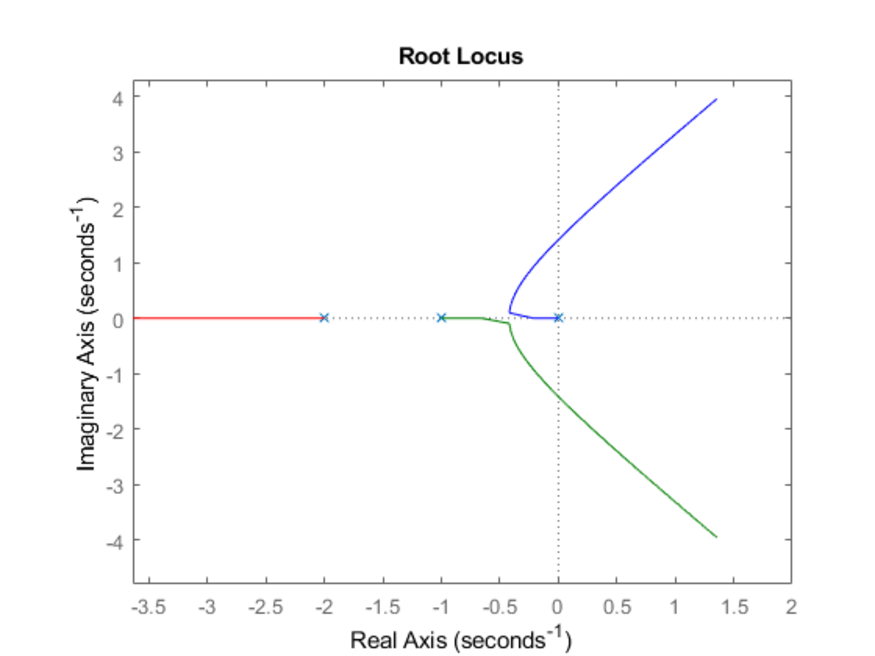
\includegraphics[scale=0.5]{rlocus1.pdf}
\end{center}
e l'andamento di quello negativo è riportato di seguito
\begin{center}
	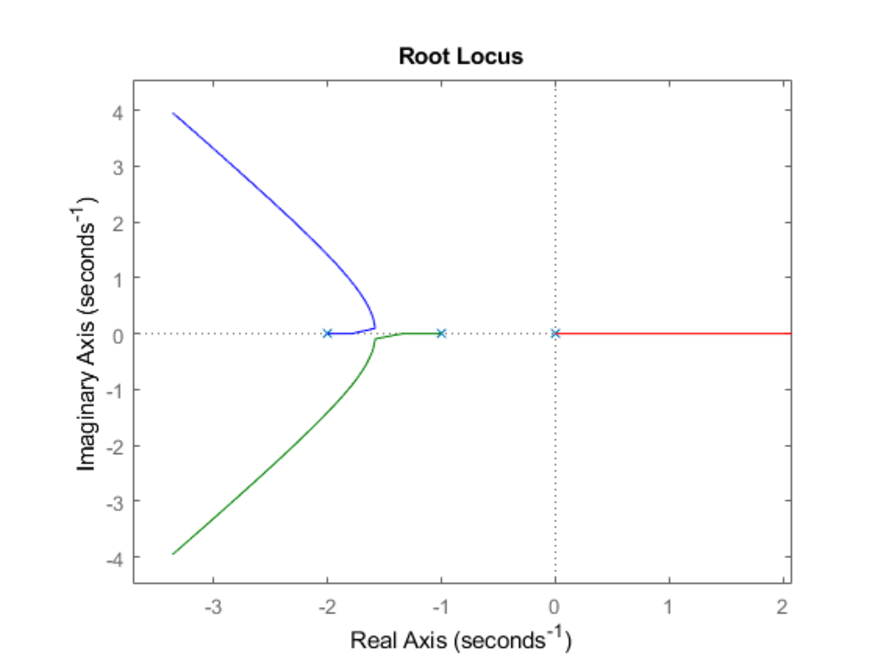
\includegraphics[scale=0.5]{rlocus2.pdf}
\end{center}
e infine riporto lo \emph{script} Matlab utilizzato 
\lstinputlisting[style=Matlab-editor]{Immagini/radici.m}

\newpage
\section{Riduzione di schemi a blocchi}
Per ricavare gli schemi del capitolo 9, partendo da quelli del capitolo 7 è necessario manipolare gli schemi a blocchi. Vediamo qualche riduzione che può tornarci utile,
\subsubsection{Spostamento di un punto di prelievo a monte di un blocco}
\begin{center}
	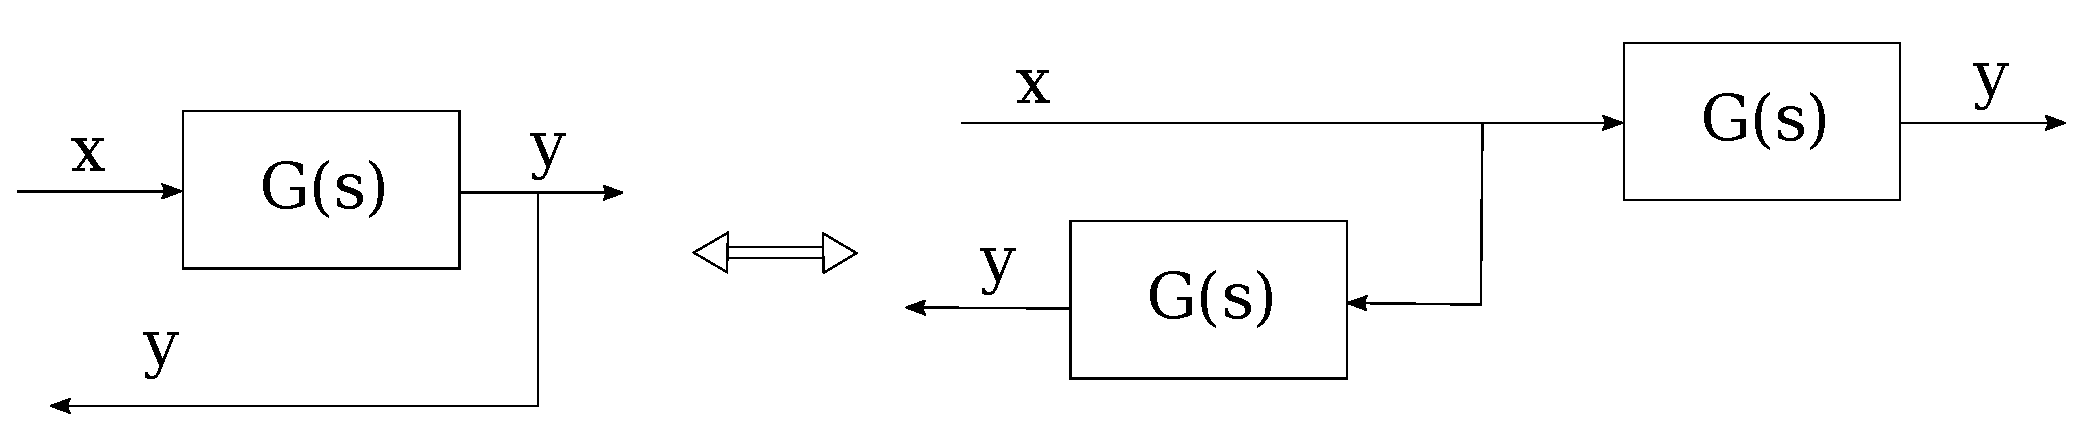
\includegraphics[scale=0.3]{riduzione4.pdf}
\end{center}

\subsubsection{Spostamento di un punto di prelievo a valle di un blocco}
\begin{center}
	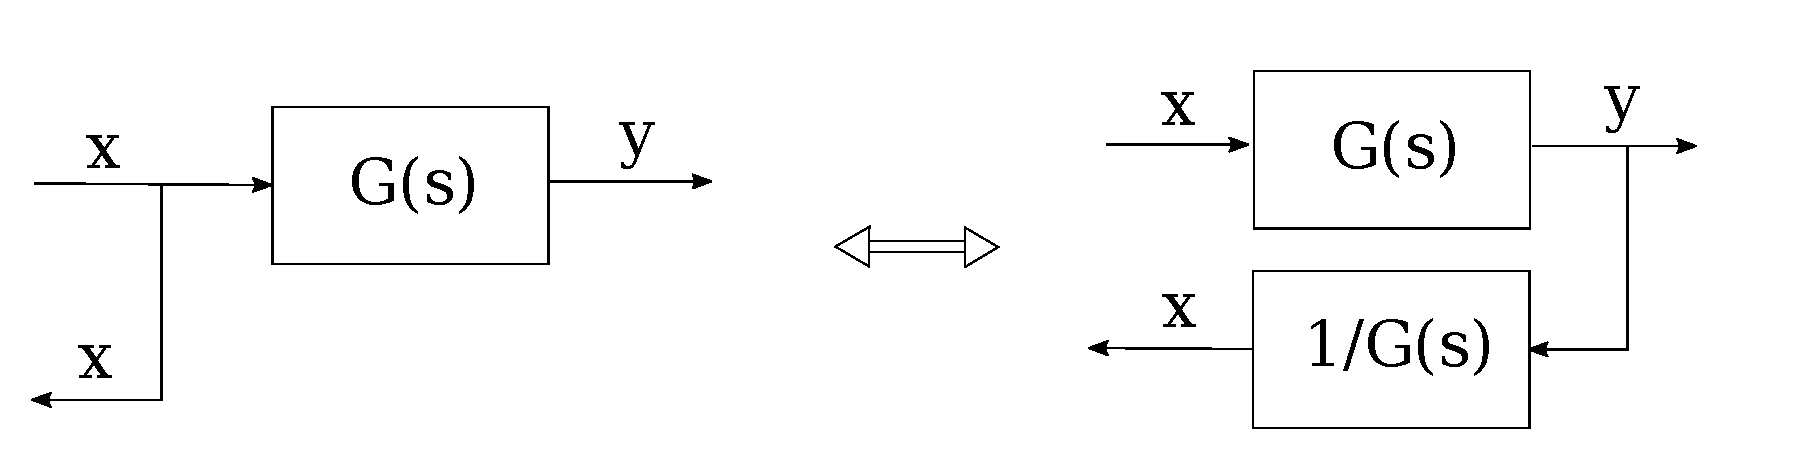
\includegraphics[scale=0.3]{riduzione5.pdf}
\end{center}

\subsubsection{Spostamento di una giunzione sommante a valle di un blocco}
\begin{center}
	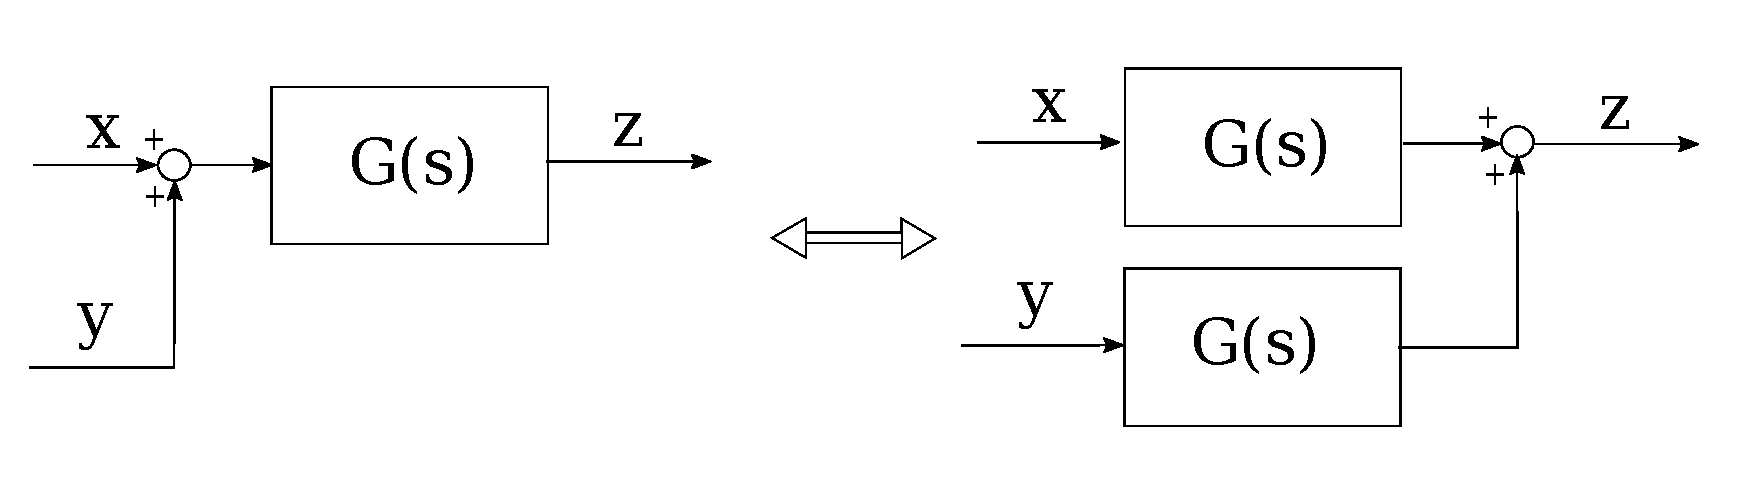
\includegraphics[scale=0.3]{riduzione6.pdf}
\end{center}

\subsubsection{Spostamento di una giunzione sommante a monte di un blocco}
\begin{center}
	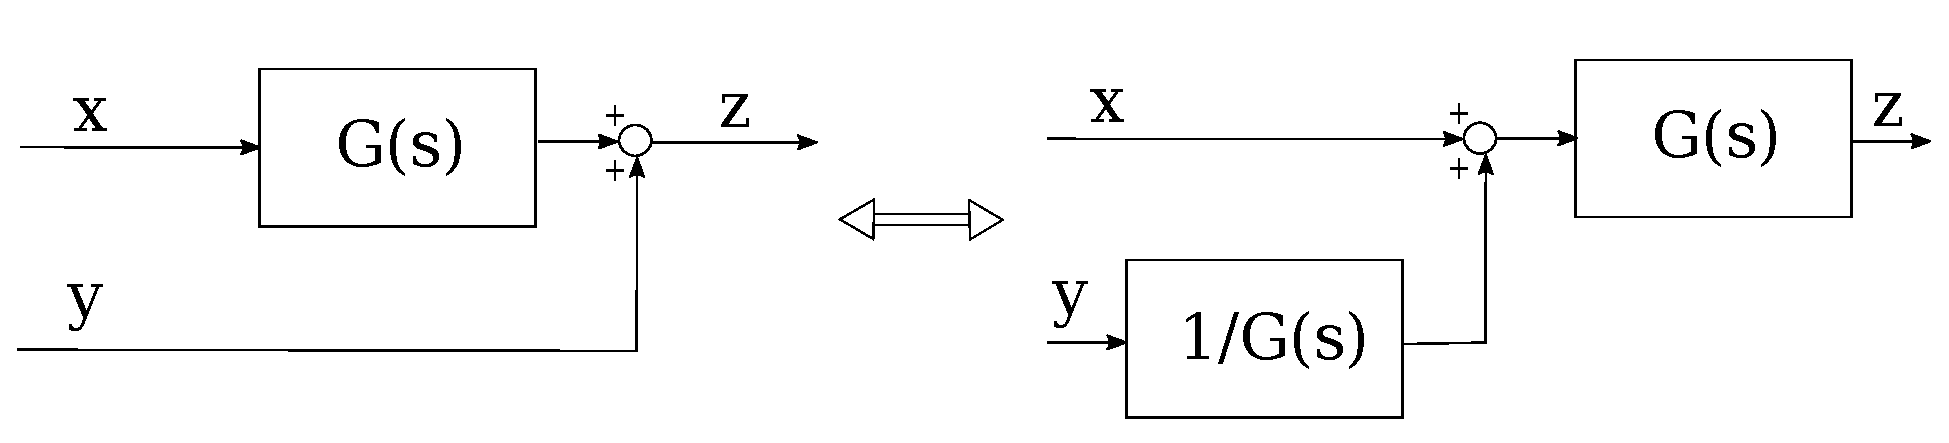
\includegraphics[scale=0.3]{riduzione7.pdf}
\end{center}